\textbf{- Reference:} 
\href{https://mysite.science.uottawa.ca/mnevins/papers/StephenHarrigan2017LWE.pdf}{Lattice-Based Cryptography and the Learning with
Errors Problem}~\cite{lattice-crypto}


$ $

Lattice-based cryptography is often considered as  post-quantum cryptography, resistant against quantum computer attacks. This section describes the mathematical hard problem that is the basis of the lattice-based cryptosystems we will explore: LWE (Learning with Error) cryptosystem, RLWE (Ring Learning with Error) cryptosystem, GLWE (General Learning with Error) cryptosystem, GLev cryptosystem, and GGSW cryptosystem.





\subsection{Overview}
\label{subsec:lattice-overview}

Suppose we have a single unknown $k$-dimensional vector $S$ as a secret key, many publicly known $k$-dimensional vectors $A^{\langle i \rangle}$.

And suppose we have a large set of the following dot products $S \cdot A^{\langle i \rangle}$: 

$S \cdot A^{\langle 0 \rangle} = s_0\cdot a_{0,0} + s_1\cdot a_{0,1} + \cdots + s_{k-1}\cdot a_{0,k-1} = b_0$

$S \cdot A^{\langle 1 \rangle} = s_0\cdot a_{1,0} + s_1\cdot a_{1,1} + \cdots + s_{k-1}\cdot a_{1,k-1} = b_1$

$S \cdot A^{\langle 2 \rangle} = s_0\cdot a_{2,0} + s_1\cdot a_{2,1} + \cdots + s_{k-1}\cdot a_{2,k-1} = b_2$

\text{ } $\vdots$


$ $

Suppose that all $(A^{\langle i \rangle}, b_i)$ tuples are publicly known. An attacker only needs $k$ such tuples to derive the secret vector $S$. Specifically, as there are $k$ unknown variables (i.e., $s_0, s_1, \cdots, s_{k-1}$), the attacker can solve for those $k$ variables with $k$ equations by using linear algebra. 

However, suppose that in each equation above, we randomly add an unknown small noise $e_i$ (i.e., error) as follows: 

$S \cdot A^{\langle 0 \rangle} = s_0\cdot a_{0,0} + s_1\cdot a_{0,1} + \cdots + s_{k-1}\cdot a_{0,k-1} + e_0 \approx b_0$

$S \cdot A^{\langle 1 \rangle} = s_0\cdot a_{0,0} + s_1\cdot a_{1,1} + \cdots + s_{k-1}\cdot a_{1,k-1} + e_1 \approx b_1$

$S \cdot A^{\langle 2 \rangle} = s_0\cdot a_{0,0} + s_1\cdot a_{2,1} + \cdots + s_{k-1}\cdot a_{2,k-1} + e_1 \approx b_2$

\text{ } $\vdots$


$ $

Then, even if the attacker has a sufficient number of $(A^{\langle i \rangle}, b_i)$ tuples, it is not feasible to derive $s_0, s_1, \cdots, s_{k-1}$, because even a small noise added to each equation prevents linear-algebra-based direct derivation of the unknown variables. For each above equation, the attacker has to consider as many possibilities as the number of the possible values of $e_i$. For example, if there are $r$ possible values of each noise $e_i$, the attacker's brute-force search space of applying linear algebra to those $n$ equations is: $\overbrace{r \times r \times r \times \cdots \times r}^{\text{n times}} = r^n$. Thus, the number of noisy equations grows, the aggregate possibilities of $e_i$s grow exponentially, which means that the attacker's cost of attack grows exponentially. 

Based on this intuition, the mathematical hard problem that constitutes lattice-based cryptography is as follows:

$ $

\begin{tcolorbox}[title={\textbf{\tboxlabel{\ref*{subsec:lattice-overview}} The LWE (Learning with Errors) and RLWE Problems}}]
\textbf{\underline{LWE Problem}}

Suppose we have a plaintext number $m$ to encrypt. The encryption formula is: $b = S \cdot A + \Delta \cdot m + e$. In this formula, $e$ is a small noise, and $\Delta$ is a scaling factor to bit-wise separate the plaintext $m$ from the noise $e$ with enough gap when they are added up (this is needed for successful decryption, which will be explained later). 

For each encryption, a random $k$-dimensional vector $A \in \mathbb{Z}_q^k$ and a small noise value $e \in \mathbb{Z}_q$ are newly sampled from $\{0, 1, \cdots, q - 1\}$, where $q$ is the ciphertext domain size. On the other hand, the $k$-dimensional secret vector $S$ is the same for all encryptions. Suppose we have an enough number of ciphertext tuples: 

$(A^{\langle 1 \rangle}, b^{\langle 1 \rangle})$, where $b^{\langle 1 \rangle} = S \cdot A^{\langle 1 \rangle} + \Delta m^{\langle 1 \rangle} + e^{\langle 1 \rangle}$ 

$(A^{\langle 2 \rangle}, b^{\langle 2 \rangle})$, where $b^{\langle 2 \rangle} = S \cdot A^{\langle 2 \rangle} + \Delta m^{\langle 2 \rangle} + e^{\langle 2 \rangle}$ 

$(A^{\langle 3 \rangle}, b^{\langle 3 \rangle})$, where $b^{\langle 3 \rangle} = S \cdot A^{\langle 3 \rangle} + \Delta m^{\langle 3 \rangle} + e^{\langle 3 \rangle}$ 

\text{ } $\vdots$

Suppose that the attacker has a sufficiently large number of $(A^{\langle i \rangle}, b^{\langle i \rangle})$ tuples. Given this setup, the following hard problems constitute the defense mechanism of the LWE (Learning with Errors) cryptosystem:

$ $

\begin{itemize}
\item \textbf{Search-Hard Problem:} There is no efficient algorithm for the attacker to find out the secret key vector $S$.
\item \textbf{Decision-Hard Problem:} We create a black box system which can be configured to one of the following two modes: (1) all $b^{\langle i\rangle}$ values are purely randomly generated; (2) all $b^{\langle i\rangle}$ values are computed as the results of $S \cdot A^{\langle i\rangle} + e^{\langle i\rangle}$ based on the randomly picked known public keys $A^{\langle i \rangle}$, randomly picked unknown noises $e^{\langle i\rangle}$, and a constant unknown secret vector $S$. Given an enough number of $(A^{\langle i \rangle}, b^{\langle i \rangle})$ tuples generated by this black box system, the attacker has no efficient algorithm to determine which mode this black box system is configured to.
\end{itemize}

$ $

These two problems are interchangeable.

$ $

\textbf{\underline{RLWE Problem}}

In the case of the RLWE (Ring Learning with Errors) problem, the only difference is that $A$, $B$, $S$, $m$, and $e$ are $(n-1)$-degree polynomials in $\mathbb{Z}_q[X] / (x^n + 1)$, and its search-hard problem is finding the unknown $n$ coefficients of the secret polynomial $S$. 

\end{tcolorbox}




\subsection{LWE Cryptosystem}
\label{subsec:lattice-scheme}

The LWE cryptosystem uses the following encryption formula: $B = S \cdot A + \Delta \cdot M + E$ (where $S$ is a secret key, $A$ is a public key randomly picked per encryption, $M$ is a plaintext, $E$ is a small noise randomly picked per encryption from a normal distribution, and $B$ is a ciphertext). $\Delta$ is a scaling factor of the plaintext $M$ (shifting $M$ by $\text{log}_2\Delta$ bits to the left). Before encrypting the plaintext, we left-shift the plaintext several bits (i.e., $\text{log}_2\Delta$ bits) in order to secure sufficient space to store the error in the lower bits.

\begin{figure}[h!]
    \centering
  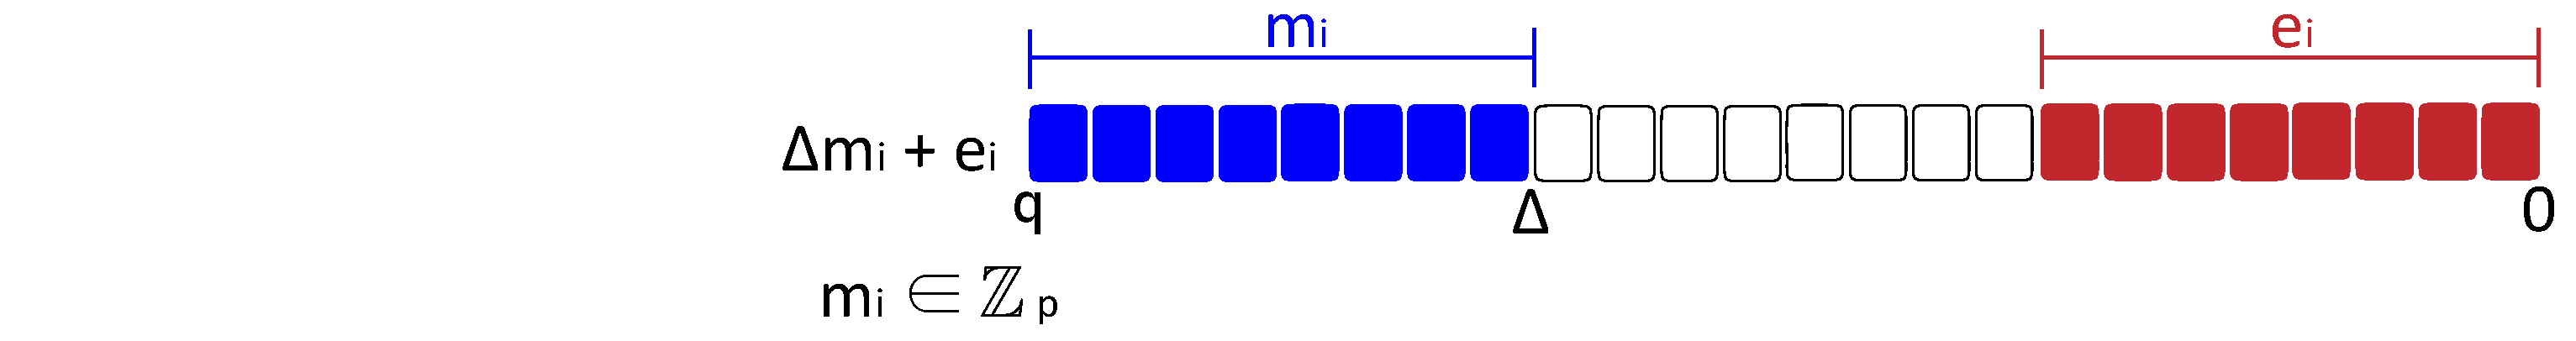
\includegraphics[width=0.8\linewidth]{figures/TFHE-fig1.pdf}
  \caption{An illustration of LWE's plaintext scaling and adding a noise: $\Delta \cdot M + E \in \mathbb{Z}_q$}
  \label{fig:scaling}
\end{figure}

\autoref{fig:scaling} visually illustrates the term $\Delta \cdot M + E$, where the plaintext $M$ left-shifted by $\text{log}_2\Delta$ bits and noised by the noise $E$. The actual encryption and decryption formulas are as follows:

\begin{tcolorbox}[title={\textbf{\tboxlabel{\ref*{subsec:lattice-scheme}} Lattice-based Cryptosystem}}]
\begin{itemize}
    \item \textbf{\underline{Encryption}: } $B^{\langle i \rangle} = S \cdot A^{\langle i \rangle} + \Delta \cdot M^{\langle i \rangle} + E^{\langle i \rangle}$, where $B^{\langle i \rangle}$ and $A^{\langle i \rangle}$ are publicly known also to the attacker, while $S, M^{\langle i \rangle}, E^{\langle i \rangle}$ are unknown (only known by the secret key owner). 

    $ $
    
    \item \textbf{\underline{Decryption}: } $ \dfrac{\lceil B^{\langle i \rangle} - S \cdot A^{\langle i \rangle} \rfloor_{\Delta}}{\Delta} = \dfrac{\lceil \Delta M^{\langle i \rangle} + E^{\langle i \rangle} \rfloor_{\Delta}}{\Delta} = M^{\langle i \rangle}$ $\Big($ provided $E{\langle i \rangle} < \dfrac{\Delta}{2}\Big )$   
\end{itemize}
\end{tcolorbox}

$\lfloor \rceil_\Delta$ means rounding the number to the nearest multiple of $\Delta$. For example, $\lfloor 16 \rceil_{10} = 20$, which is rounding 16 to the nearest multiple of 10. As another example, $\lfloor 17 \rceil_{8} = 16$, which is rounding 17 to the nearest multiple of 8 (note that 17 is closer to 16 than 24, thus it is rounded to 16). 


$ $

\noindent \textbf{Correctness: } In the decryption scheme, computing $B^{\langle i \rangle} - S \cdot A^{\langle i \rangle}$ gives $\Delta \cdot M^{\langle i \rangle}+ E^{\langle i \rangle}$, which is \autoref{fig:scaling}. Then, $\lceil \Delta \cdot M^{\langle i \rangle} + E^{\langle i \rangle} \rfloor_{\Delta}$ (i.e., rounding the value to the nearest multiple of $\Delta$) gives $\Delta \cdot M^{\langle i \rangle}$, provided the added noise $E^{\langle i \rangle} < \frac{\Delta}{2}$. That is, if the noise is less than $\frac{\Delta}{2}$, it will disappear during the rounding. Finally, right-shifting $\Delta \cdot M^{\langle i \rangle}$ by $\text{log}_2 \Delta$ bits gives $M^{\langle i \rangle}$. To summarize, if we ensure $E^{\langle i \rangle} < \frac{\Delta}{2}$ (which is why the noise $E^{\langle i \rangle}$ should be smaller than this threshold), then we can blow away $E^{\langle i \rangle}$ during the decryption's rounding process and retrieve the original $\Delta \cdot M^{\langle i \rangle}$. The reason we scaled $M^{\langle i \rangle}$ by $\Delta$ is to: (i) create the space for storing $E^{\langle i \rangle}$ in the lower bits during encryption such that the noise bits do not interfere with the plaintext bits (to avoid corrupting the plaintext bits); and (ii) blow away the noise $E^{\langle i \rangle}$ stored in the lower bits during decryption without corrupting the plaintext $M^{\langle i \rangle}$. 

$ $

\noindent \textbf{Security: } Given an attacker has a large list of $(A^{\langle i \rangle}, B^{\langle i \rangle})$ (i.e., many ciphertexts), it's almost impossible for him to derive $S$, because of the random noise $E^{\langle i \rangle}$ added in each encryption (which is a search-hard problem described in \autoref{subsec:lattice-overview}). This is because even small added unknown noises $E^{\langle i \rangle}$ greatly change the mathematical solution for $S$ that satisfies all the $B^{\langle i \rangle} = S \cdot A^{\langle i \rangle} + \Delta \cdot M^{\langle i \rangle} + E^{\langle i \rangle}$ equations. 

%$Y = S \cdot X$

Even in the case that the attacker has a large list of $(A^{(j)}, B^{(j)})$ generated for the same ciphertext $M^{\langle i \rangle}$ (where each ciphertext used different $A^{(j)}$ and $E^{(j)}$ to encrypt the same $M^{\langle i \rangle}$), he still cannot derive $M^{\langle i \rangle}$, because a randomly picked different noise $E^{(j)}$ is used for every $(A^{(j)}, B^{(j)})$ and gets accumulated over ciphertexts, which exponentially complicates the difficulty of the linear algebra of solving $S$. Also, in the actual cryptosystem (\autoref{sec:lwe}), the public key $A^{\langle i \rangle}$ and the secret key $S$ are not a single number, but a long vector comprising many random numbers. Thus, adding $A^{\langle i \rangle }\cdot S$ to $\Delta M^{\langle i \rangle} + E^{\langle i \rangle}$ adds a higher entropy of randomness against the attack. 

$ $

To summarize, the lattice-based cryptography hides a plaintext by adding the encryption component $S \cdot A$ to it as well as a small random noise $E$. During decryption, the secret key owner re-creates this encryption component $A \cdot S$ by using her $S$ and removes it, and then also removes the noise $E$ by the rounding technique, and finally right-shifts the remaining $\Delta M$ by $\text{log}_2 \Delta$ bits to get $M$.

\subsection{RLWE Cryptosystem}

In the RLWE cryptosystem, the formula in \tboxlabel{\ref*{subsec:lattice-scheme}} is the same, but $S, A^{\langle i \rangle}, M^{\langle i \rangle}, E^{\langle i \rangle}$ are polynomials. 